\documentclass[oneside]{article}%You can define the type of paper here.
%%Useful packages that I commonly use.
%\usepackage[numbers]{natbib}%Bibliography package (help at http://merkel.zoneo.net/Latex/natbib.php).
%\usepackage{url}%Package to highlight url.
\usepackage{mathpazo}%Sets font to be math pazo.
\usepackage{alltt}%Allows the use of verbatim (good for printing out code).
%\usepackage{graphicx}%Used to import images.
\usepackage{amsmath, amssymb, amscd}%Contains the AMS expanded math symbols library.
\usepackage[explicit]{titlesec} %To remove section title in headers
%%For those who want smaller margins, you can use this:
\usepackage[top=1in, bottom=1in, left=1in, right=1in]{geometry}
\usepackage{fancyhdr} %%For headers/footers
%\usepackage{savetrees} %%Removes white space
\pagestyle{fancy} %%For fancy headers
\usepackage{tocloft}
\renewcommand{\cftsecleader}{\cftdotfill{\cftdotsep}}
\usepackage{pdfpages}
\usepackage{graphicx} %for including graphics and figures
\usepackage{enumerate} %for custom enumerations
\usepackage{caption} %for captions outside of floats
\usepackage{chemarr} %for using xrightleftharpoons for chemical reactions
\usepackage{multirow} % for using a table label that is multiple rows in size

\fancyhf{} %removes page enumeration from center middle of footer

\def\undertilde#1{\mathord{\vtop{\ialign{##\crcr
   $\hfil\displaystyle{#1}\hfil$\crcr\noalign{\kern1.5pt\nointerlineskip}
   $\hfil\tilde{}\hfil$\crcr\noalign{\kern1.5pt}}}}}


%for an approximate proportion symbol:
\def\approxprop{%
  \def\p{%
    \setbox0=\vbox{\hbox{$\propto$}}%
    \ht0=0.6ex \box0 }%
  \def\s{%
    \vbox{\hbox{$\sim$}}%
  }%
  \mathrel{\raisebox{0.7ex}{%
      \mbox{$\underset{\s}{\p}$}%
    }}%
}

\begin{document}
%% Top needs  to say "UNIVERSITY OF MONTANA: COMPUTER SCIENCE DEPARTMENT"
%%Title
\fancyhead[L]{CSCI 576 - HUMAN-COMPUTER INTERACTION} %%Header
\fancyhead[R]{\thepage} %Page enumeration
\fancyfoot[L]{BLAIR GEMMER - UNIVERSITY OF MONTANA: COMPUTER SCIENCE DEPARTMENT} %Footer
\rhead{}
\fancyhead[R]{\thepage} %Page enumeration
\renewcommand{\footrulewidth}{1pt}

%Fix headers on Table of Contents and List of Figures:
\fancypagestyle{plain}{
\fancyhead{}
\fancyfoot{}
\fancyhead[L]{CSCI 576 - HUMAN-COMPUTER INTERACTION} %%Header
\fancyfoot[L]{BLAIR GEMMER - UNIVERSITY OF MONTANA: COMPUTER SCIENCE DEPARTMENT} %Footer
\rhead{}
\renewcommand{\footrulewidth}{1pt}
}

\title{Project 4: Reflection on User-Testing}
\author{Blair Gemmer}
\maketitle

\newcommand*\Hide{%
\titleformat{\chapter}[display]
  {}{}{0pt}{\Huge}
\titleformat{\part}
  {}{}{0pt}{}
}

\newpage
User testing went better than expected actually. Each user arrived at the perfect time, so there
wasn’t a lot of waiting around or users piling up at the door. All the equipment was ready to use
and we didn’t run out of battery power or having any major catastrophes.\\

We really got a lot of good feedback, as well. The videos showed a ton of information we
missed by merely observing and taking notes. The users were really good about saying
what they were thinking and generally commenting and asking questions that provided good
feedback. If we had infinite time, there could be many new features or bug fixes based on the
many excellent comments and questions the users provided.\\

That being said, there were many unexpected things that I personally didn’t think the users
would have difficulty with that they found quite difficult. Simple things like how to place towers
and navigate the menu system seemed like they weren’t very intuitive to the user.\\

Overall, I think the most useful feedback was from the questionnaires and the video recording.
Seeing from the user’s perspective really made it feel like we were sitting in the user’s chair,
seeing the game for the first time.\\

\textbf{Some examples of interesting questions and comments from the users:}\\

\begin{enumerate}
	\item I don't understand the tower on the bottom, maybe it's the cost?
	\item We've built the giant castle of survivors!
	\item Do I have to kill the zombies?
	\item *User tries for a few minutes to swipe a screen that should be pressed.*
	\item There's really no point to this game once you fill the screen with towers.
\end{enumerate}
%for creating a table (notice the multicolumn and multirow commands also for formatting the labels)
%\begin{center}
%	\begin{tabular}{| l | l | l | l | l |}
%		\hline
%		\multirow{3}{*}{Day \#}  & \multicolumn{4}{c}{Mean density}\vline\\
%		\cline{2-5}
%		& \multicolumn{2}{c}{In isolation} \vline& \multicolumn{2}{c}{In competition}\vline\\
%		\cline{2-5}
%		& \textit{P. aurelia} & \textit{P. caudatum} & \textit{P. aurelia} & \textit{P. caudatum}\\
%		\hline
%		0 & 2 & 2 & 2 & 2\\
%		\hline
%		1 & | & | & | & |\\
%		\hline
%		2 & a & b & c & d\\
%		\hline
%	\end{tabular}
%	\captionof{table}{Summary of the cases shown in Figure 3.}
%\end{center}

%for creating a vector or matrix, floating to the left:
%$f(x) =$ \( \left[ \begin{array}{ccc}
%a&b&c\\
%d&e&f
%\end{array} \right]\) 
%
%%for creating a vector or matrix, floating to the right:
%$f(x) =$ \[ \left[ \begin{array}{ccc}
%a&b&c\\
%d&e&f
%\end{array} \right]\] 

%For creating an image with a caption:
%\begin{minipage}{\linewidth}
%		\makebox[\linewidth]{%
%		\centering
%		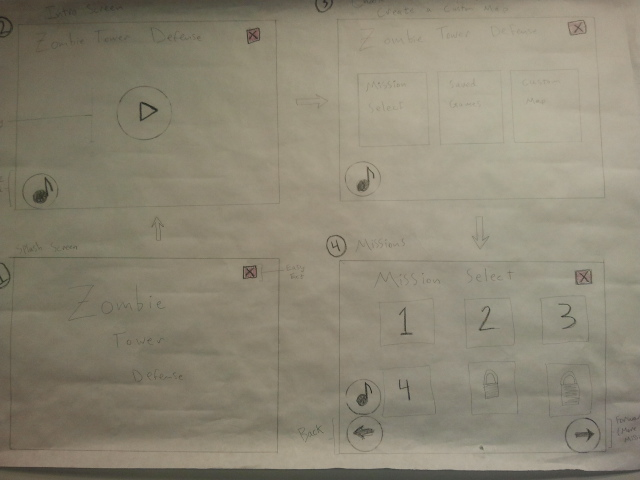
\includegraphics[scale=.1]{plots/problem242/1.jpg}}
%		\captionof{figure}{Plot of $a_n$ along time $n$, showing the oscillation between $a_{max}$ and $a_{min}$, }
%		\captionof*{figure}{where $a_{max} = $ toxicity of a drug and $a_{min} = $ effectual level of drug.}
%		\end{minipage}\\


\end{document}